\documentclass[11pt]{article}
\addtolength{\oddsidemargin}{-1.cm}
\addtolength{\textwidth}{2cm}
\addtolength{\topmargin}{-2cm}
\addtolength{\textheight}{3.5cm}

\usepackage[pdftex]{graphicx}
\usepackage{hyperref}
\usepackage{cite}
\hypersetup{
    colorlinks=true,
    linkcolor=black,
    filecolor=magenta,      
    urlcolor=cyan,
}

% define the title
\author{Team Bravo}
\title{Assignment 1 Software Requirements Specification and Technology Neutral Process Design}
\begin{document}
\setlength{\parskip}{6pt}

% generates the title
\begin{titlepage}
	
	\begin{center}
		% Upper part of the page       
		
\includegraphics[width=1\textwidth]{../Diagrams/Images/University_of_Pretoria_Logo.PNG}\\[0.5cm]    
		\textsc{\LARGE Department of Computer Science}\\[0.5cm]
		\textsc{\Large COS 301}\\[0.5cm]
		\textsc{\Large Mini Project} \nocite{ref}\\[0.5cm]
		% Title
		\rule{\linewidth}{0.5mm} \\[0.4cm]
		{ \huge \bfseries Software Requirements Specification and Technology Neutral Process Design and Software Architecture Documentation}\\[0.2cm]
		\rule{\linewidth}{0.5mm} \\[1cm]
		
		% Author and supervisor
		\textsc{\Large Team Bravo}\\[1cm]
		
		
		\begin{minipage}{0.4\textwidth}
			\begin{flushleft} \large
				\emph{Student:}\\[0.75cm]
				Daniel {King}
			\end{flushleft}
		\end{minipage}
		\begin{minipage}{0.4\textwidth}
			\begin{flushright} \large
				\emph{Student number:} \\[0.75cm]
				u13307607
			\end{flushright}
		\end{minipage}
		
		
		\begin{minipage}{0.4\textwidth}
			\begin{flushleft} \large
				\emph{} \\
				Azhar {Mohungoo }
			\end{flushleft}
		\end{minipage}
		\begin{minipage}{0.4\textwidth}
			\begin{flushright} \large
				\emph{} \\
				u12239799
			\end{flushright}
		\end{minipage}
		
		
		\begin{minipage}{0.4\textwidth}
			\begin{flushleft} \large
				Andreas {du Preez}
			\end{flushleft}
		\end{minipage}
		\begin{minipage}{0.4\textwidth}
			\begin{flushright} \large
				\emph{} \\
				u12207871 
			\end{flushright}
		\end{minipage}
		
		
		\begin{minipage}{0.4\textwidth}
			\begin{flushleft} \large
				Banele {Nxumalo}
			\end{flushleft}
		\end{minipage}
		\begin{minipage}{0.4\textwidth}
			\begin{flushright} \large
				\emph{} \\
				u12201911 
			\end{flushright}
		\end{minipage}
		
		
		\begin{minipage}{0.4\textwidth}
			\begin{flushleft} \large
				Frederic {Ehlers}
			\end{flushleft}
		\end{minipage}
		\begin{minipage}{0.4\textwidth}
			\begin{flushright} \large
				\emph{} \\
				u11061112  
			\end{flushright}
		\end{minipage}
		
		
		\begin{minipage}{0.4\textwidth}
			\begin{flushleft} \large
				Diana {Obo}
			\end{flushleft}
		\end{minipage}
		\begin{minipage}{0.4\textwidth}
			\begin{flushright} \large
				\emph{} \\
				u13134885
			\end{flushright}
		\end{minipage}
		
		
		\begin{minipage}{0.4\textwidth}
			\begin{flushleft} \large
				Bilal {Muhammad}
			\end{flushleft}
		\end{minipage}
		\begin{minipage}{0.4\textwidth}
			\begin{flushright} \large
				\emph{} \\
				u13080335
			\end{flushright}
		\end{minipage}
		\vfill
		
	\end{center}
\end{titlepage}

\renewcommand{\thesection}{\arabic{section}}
\newpage

\tableofcontents

\textsc{}\\[1cm]

\begin{center}
\textsc{\Large Bravo github repository link}\\[0.5cm]
For further references, please click on this \href{https://github.com/ish1993/Bravo}{link}.
\end{center}

\newpage

\section{Introduction}

This document aims to specify the functional and non-functional requirements of a document archiving system, as specified by Ms Vreda Pieterse of the Computer Science Department.

It will serve as a means of communication between the client and developers as well as providing an elaboration and a clear discription of it's implementation specifications.

\section{Vision}

We intend to create a system that will allow authors and their co-authors to work on their research papers in an environment that reassures collaborative work, which in turn diminishes the time spent on papers with multiple authors. The following are what we plan to achieve: 

\begin{itemize}
	\item Keep track of research papers.
	\item View meta-data of research papers. 
	\item Allow multiple authors to collaborate on the same research paper. 
	\item Different levels of authority, i.e. Admin, (Co)Author, User.
	\item View and edit the details, of a text based profile, of different researchers. 
	\item Implemention as a website and an android application.
\end{itemize} 

\section{Background}

We live in a world where time is valuable. We would like to do as much as we possibly can in the shortest amount of time. And if that's not possible, we work in teams to ensure that we achieve that goal. 

Reseacher papers tend to be fairly lengthy, and if completed by only one author, it could be quite a tedious process. Hence we propose a system which would make the storage and collaboration of research articles and papers effortless by producing an archive system.

\newpage

\section{Architecture Requirements}

\subsection{Access channel requirements}
The different access channels for the system will be as follows:

\subsubsection{Web Application}
The system can be used via a web application that uses RESTful web services and bootstrap technology. The system will be fully supported on the following web browsers:

\begin{itemize}
	\item Chrome 7.0.517 and up
	\item Firefox 3.6 and up
	\item Safari 4 and up
	\item Edge
\end{itemize}

Bootstrap will be used so that the web application will also be accessible by mobile web browsers that support HTML5 and JavaScript technology.

\subsubsection{Mobile Application}
The system will also be accessible via a mobile application and will be operational on the following mobile operating systems:

\begin{itemize}
	\item Android 4.0 (Ice Cream Sandwich) and up.
\end{itemize}

\subsection{Quality requirements}

\begin{itemize}
	\item Security - The system shall identify all of its client applications before allowing them access to those enities. Possible measurement methods: Success rate in authentication, percentage of successful attacks, encryption level and probability/time/resources needed to attack the system.
	\item Usability - The degree of ease of use and training needed for end users. Possible measurement methods: Time it took a user to find a report (search functionality), percentage of deadlines met (notification functionality) and time it took a user to perform certain tasks.
	\item Auditability - The degree to which transactions can be traced. Possible measurement methods: The number and precision of logs generated in a period of time (metadata accessed/deleted/added).
	\item Portability - Measure ability of the system to run under different computing environments. Possible measurement methods: Number of targeted software environments (ie different browsers and operating systems) and proportion of platform specific functionality.
	\item Maintainability - Measures ability to make changes quickly and cost effectively. Possible measurement methods: Degree of complexity to make changes to the format of the metadata and mean time to add or change certain functionalities (ie new report types and new types of users).
	\item Availability - Percentage of time that the system is up and running correctly. Possible measurement methods: Length of time between failures and length of time needed to resume operation after a failure.
	\item Performance - Possible measurement methods: How well the system perform under high workload and number of events processed/denied in some interval of time.
\end{itemize}

\subsection{Integration requirements}

	\subsubsection{Integration channels}
		\begin{itemize}
			\item System will be integrated on two platforms: a website and an android application.
		\end{itemize}
	
	\subsubsection{Protocols}
		\begin{itemize}
			\item Protocols needed for the website:  HTTPS, Data Query Protocol
			\item Protocols needed for the application: Session Initiation Protocol (SIP)
		\end{itemize}
	
	\subsubsection{API specification (UML form) and technology specific API specification}
		\begin{itemize}
			\item UML diagram here
		\end{itemize}
	
	\subsubsection{Integration quality requirements}
		\begin{itemize}
			\item Reliability - The service must not crash, it must run effectively and efficiently allowing users to make use of the service at all times.
			\item Auditability - Have logs record all activity that occurs thus all actions and occurrences can be traced.
			\item Security - Giving the users reassurance that the system will protect their details and content. Allow secure and safe communication between user and the system.
			\item Maintainability - Provide easy, effective and efficient maintenance to the system allowing minimal or no downtime of the system.
			\item Usability - Allow users to use the system with ease and minimal need for tutorials. Ensure that the system is self-explanatory, efficient and effective. 
			\item Portability - To provide compatibility with as many systems as possible without integration failure or function failure.
			\item Availability - Minimise downtime of the system. Quick recoveries from crashes, preventive measures to minimise chances of system crash.
			\item Performance - The rate of work done when the system has either a high or low workload and minimise amount of denied events. 
			\item Seamless transitions between platforms - Implementation between the integrated platforms must not vary greatly to avoid confusion and allow ease of use. 
		\end{itemize}

\subsection{Architecture constraints}

\begin{itemize}
	\item The platform must exist in 2 mediums, namely web and android application.
	\item It is an internal network to be used by the Computer Science department, so it need not to source any information from the web.
	\item Any form of database can be used, but the team has decided that MySQL would be the best option from the current skillset.
	\item PHP and JavaScript will be used for the web and Android Studio for the android application.
	\item The system should cater for and including 100 users as a maximum.
	\item There should be a log that records all activity on the system
\end{itemize} 

\newpage

\section{Functional requirements and application design}

\subsection{Use case prioritization}
This section specifies the level of importance of different use cases, prioritized in terms of the following 3 catogories: Critical, Important and Nice-To-Have. Each of which has a lesser importance than the previous one.

\subsubsection{Critical:}
	\begin{itemize}
		\item Server connection
		\item Database connection
		\item User gateaway
		\begin{itemize}
			\item Login user
			\item Register user
			\item Authenticate user
		\end{itemize}
		\item Research paper management
		\begin{itemize}
			\item View paper
			\item Modify paper
			\item Publish paper
			\item Assign venue for paper
			\item View research paper venue
		\end{itemize}
		\item User account management
		\begin{itemize}
			\item Create new account
			\item Edit account
			\item Remove account
			\item View user account
		\end{itemize}
		\item Log services
		\begin{itemize}
			\item View statistics of person,group or department ( e.g number of units,publications etc)
			\item View recent activities of users
		\end{itemize}:
			\item Other
		\begin{itemize}
			\item System should be able to keep track of research.
		\end{itemize}
		\begin{itemize}
			\item System should only allow one primary user and the rest are co-authors. There shouldn’t be a time where there is no primary user or more than one primary user
		\end{itemize}
		\begin{itemize}
			\item There should exist a super user (limited to one only), which is higher than the admin. This user will be in charge of everything and anything and should be able to give and withdraw admin privileges from any user.
		\end{itemize}
		\begin{itemize}
			\item No documents are to be posted, only metadata such as: Progress bars, status of research (accepted/rejected), etc.
		\end{itemize}
		\begin{itemize}
			\item Research documents cannot be deleted but archived.
			
		\end{itemize}
	\end{itemize}
	
\subsubsection{Important:}	
	\begin{itemize}
		\item Notification Services
		\begin{itemize}
			\item Set deadline
			\item Extend deadline
		\end{itemize}
	
		\item Archival Services
		\begin{itemize}
			\item Backup  database
			\item Retrieve backed up information
		\end{itemize}
	\end{itemize}
	\begin{itemize}
		\item HOD is able to see everything is their department.
		\item One user can belong to multiple research groups.
		\item Deadline notifications should be sent to all relevant members via email.
		\item Publication details like, title, authors, use of research intended venue.
		\item Users should be able to keep track of their units that they have accumulated.
	\end{itemize} 
	
\subsubsection{Nice-To-Have:}
	\begin{itemize}
		\item ???
	\end{itemize}

\subsection{Use case/Services contracts}
\begin{itemize}
	\item Server Connection
\end{itemize}

{\raggedright
	\textbf{Description: }The ability for a user to make a connection to the server
}

{\raggedright
	\textbf{Pre-Condition: }The user must be attempting to begin using the service
	and must not be already using it.
}

{\raggedright
	\textbf{Post-Condition:} The service must now be displayed to the user and an
	option to login must be available.
}

\begin{itemize}
	\item Database Connection
\end{itemize}

{\raggedright
	\textbf{Description: }The ability for the program to connect to the database.
}

{\raggedright
	\textbf{Pre-Condition: }The program must be in a state where database connection
	is required. Eg a user is attempting to login to the system
}

{\raggedright
	\textbf{Post-Condition: }The program should be able to interact with the
	database at this point.
}

\begin{itemize}
	\item User gateway
\end{itemize}

{\raggedright
	\textbf{Description: }The ability for a user to login to the system
}

{\raggedright
	\textbf{Pre-Condition: }The user must have provided login details that match
	those found in the database system.
}

{\raggedright
	\textbf{Post-Condition: }The user must be considered “logged in” by the system.
}

\begin{itemize}
	\item Research paper management
\end{itemize}

{\raggedright
	\textbf{Description: }The ability to interact with the research paper eg
	edit/delete it
}

{\raggedright
	\textbf{Pre-Condition: }A research paper must be specified
}

{\raggedright
	\textbf{post-Condition: }The research paper needs be modified in the desired
	way.
}

\begin{itemize}
	\item User Account Management
\end{itemize}

{\raggedright
	\textbf{Description: }The user should be able to view and edit his account details
}

{\raggedright
	\textbf{Pre-Condition: }The user must be considered logged in
}

{\raggedright
	\textbf{Post-Condition: }The user has edited part of his profile, or is able to see the details regarding his profile.
}

\begin{itemize}
	\item Log services
\end{itemize}

{\raggedright
	\textbf{Description: }The ability for logs to be created of the work done on the various papers
}

{\raggedright
	\textbf{Pre-Condition: }A paper must be edited or otherwise modified in some way
}

{\raggedright
	\textbf{Post-Condition: }The action is recorded in a log
}

\begin{itemize}
	\item Notificaiton Service
\end{itemize}

{\raggedright
	\textbf{Description: }The ability to notify the user of various actions that have taken place on a paper they are an author of
}

{\raggedright
	\textbf{Pre-Condition: }The paper has been modified in some way, and the user must be an author of said paper
}

{\raggedright
	\textbf{Post-Condition: }An email is sent to the user notifying him/her
}

\begin{itemize}
	\item Search Services
\end{itemize}

{\raggedright
	\textbf{Description: }The ability to search for papers that will be presented at the same conference.
}

{\raggedright
	\textbf{Pre-Condition: }There must exist papers within the database that are related in that way.
}

{\raggedright
	\textbf{Post-Condition: }The paper/s in question are displayed for the user.
}

\begin{itemize}
	\item Archival Services
\end{itemize}

{\raggedright
	\textbf{Description: }The ability to find all papers worked on, or currently being worked on
}

{\raggedright
	\textbf{Pre-Condition: }The user doing so must be the head of department also the paper in question must exist in the database.
}

{\raggedright
	\textbf{Post-Condition: }The paper being searched is displayed for the user.
}

\subsection{Required functionality}

\newpage

\subsection{Process specifications}

\subsubsection{Server Connection}
\begin{center} 
	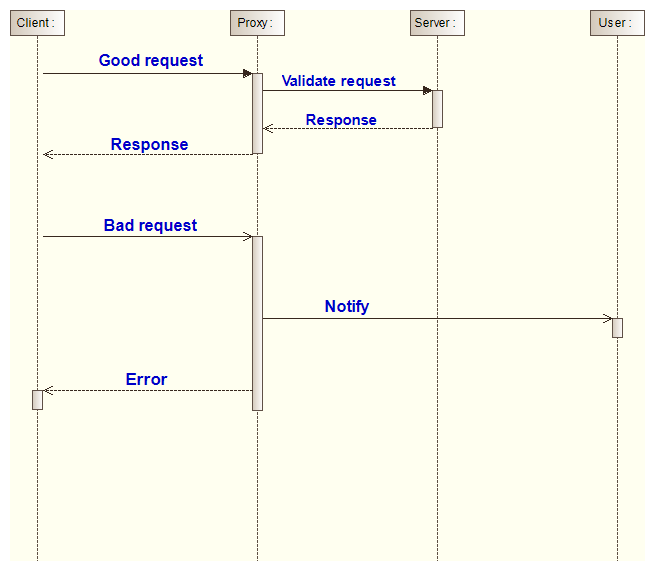
\includegraphics[width=\textwidth]{../Images/Server_Connection_Sequence_Diagram.png}\\[0.5cm]
\end{center}

\newpage
\subsubsection{Database Connection}
\begin{center} 
	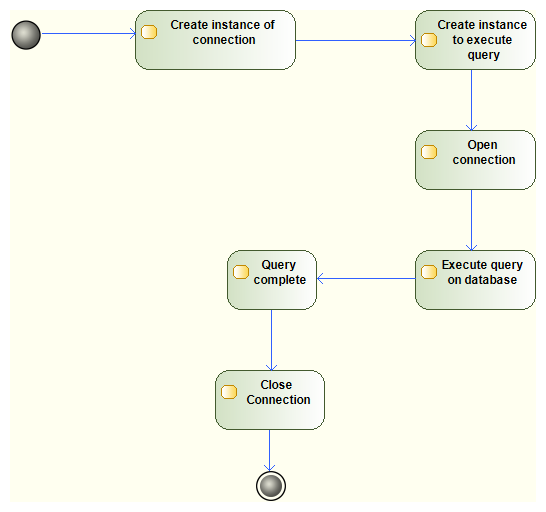
\includegraphics[width=\textwidth]{../Images/Database_Connection_Activity-Diagram.png}\\[0.5cm]
\end{center}

\newpage
\subsubsection{Login}
\begin{center} 
	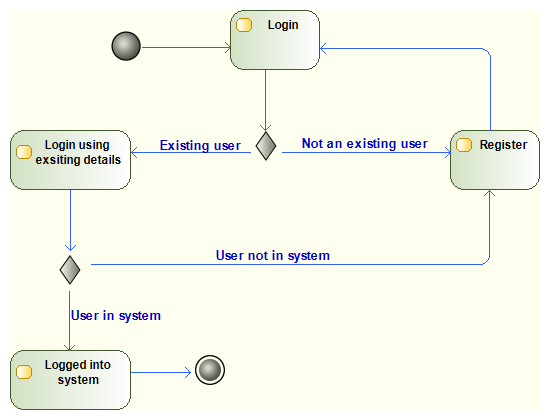
\includegraphics[width=\textwidth]{../Images/Login_Activity_Diagram.png}\\[0.5cm]
\end{center}

\newpage
\subsubsection{Logout}
\begin{center} 
	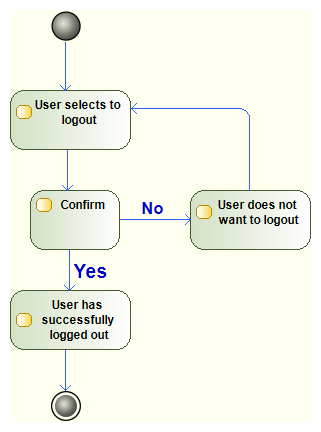
\includegraphics[width=\textwidth]{../Images/Logout_Activity_Diagram.png}\\[0.5cm]
\end{center}

\newpage
\subsubsection{New Author}
\begin{center} 
	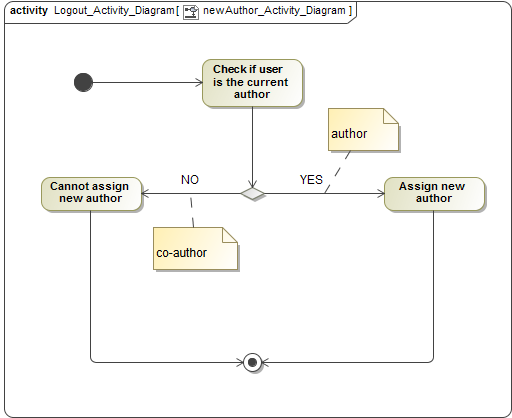
\includegraphics[width=\textwidth]{../Images/newAuthor_Activity_Diagram.png}\\[0.5cm]
\end{center}

\subsection{Domain Model}
\begin{center}
	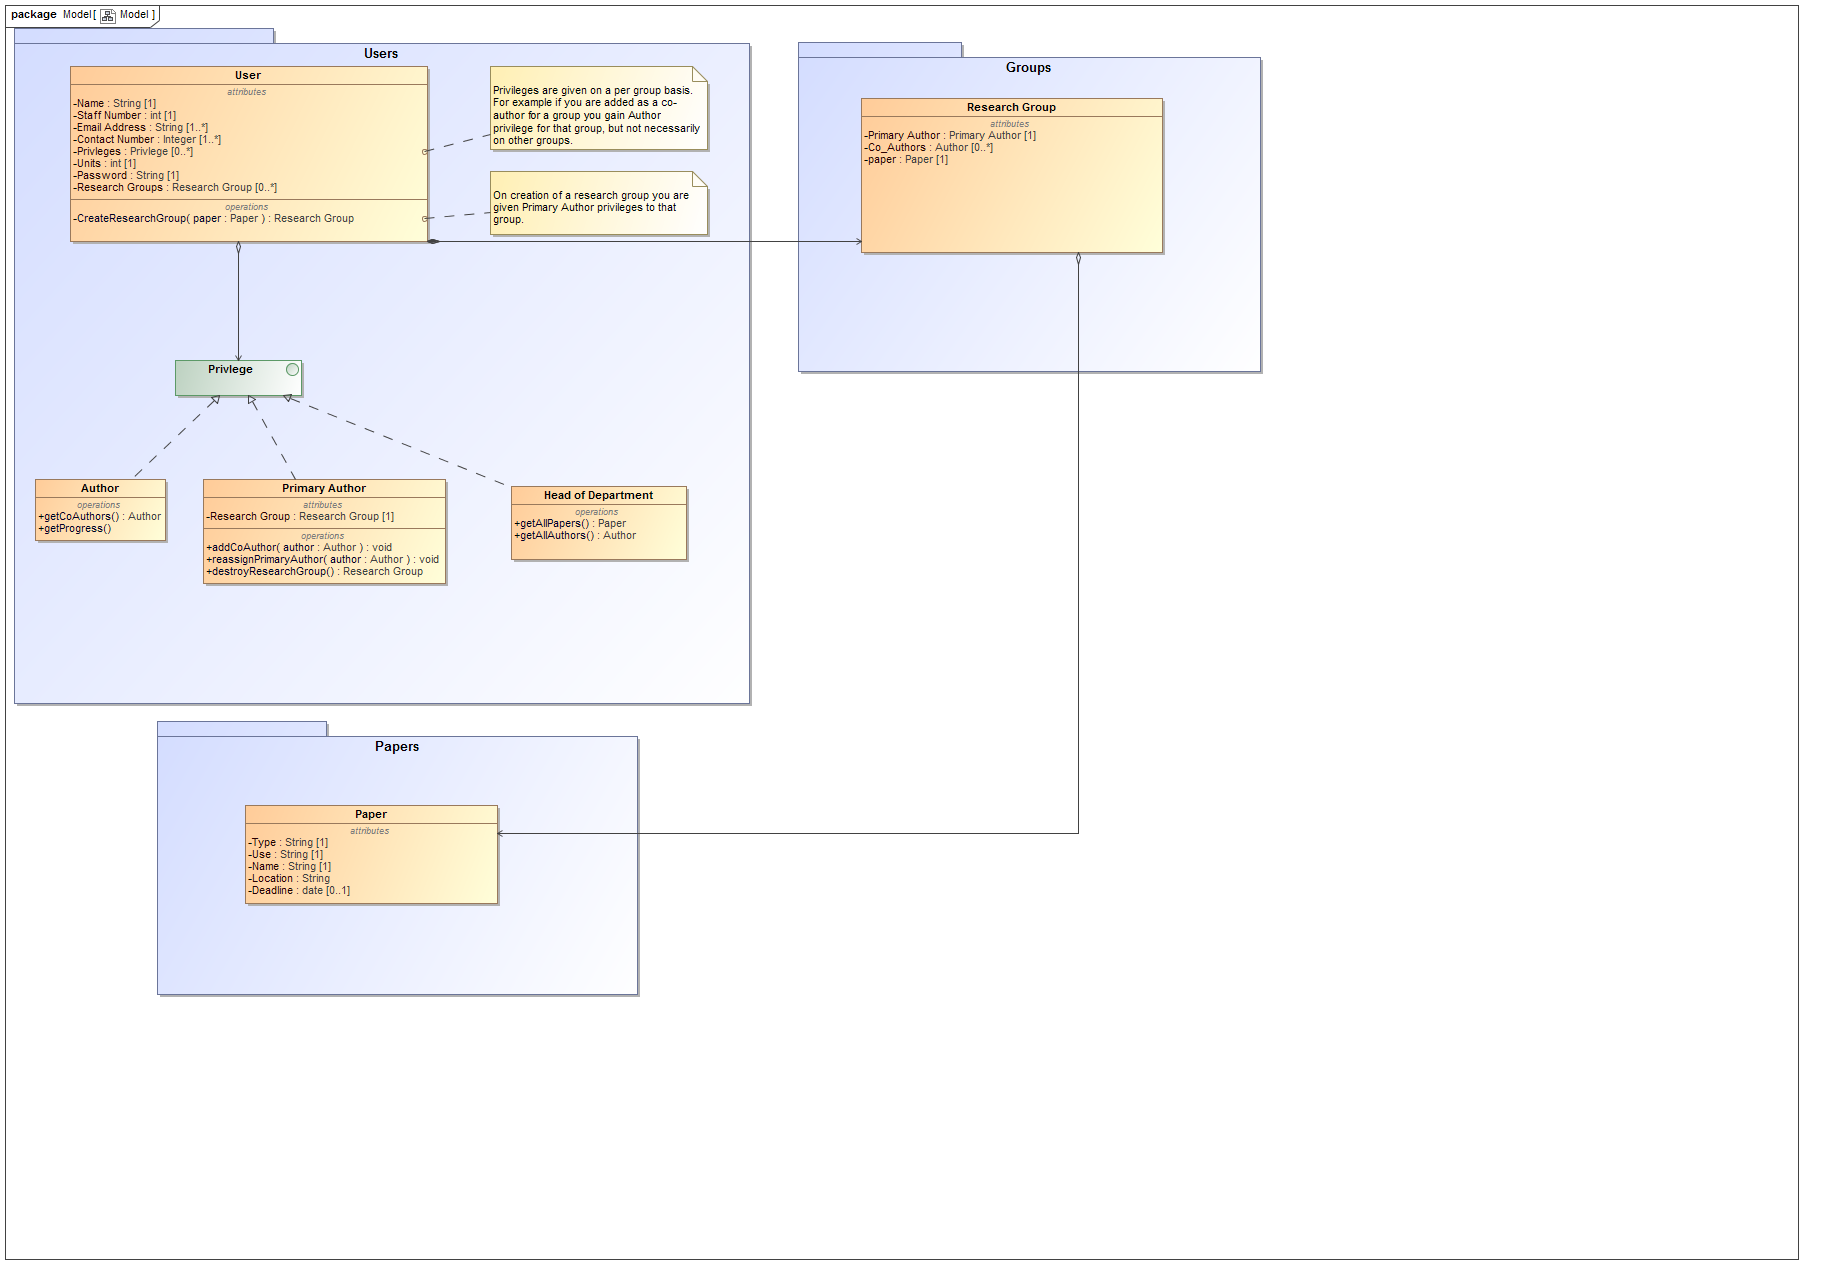
\includegraphics[width=\textwidth]{../Images/DomainModel.png}\\[0.5cm]
\end{center}

\section{Open Issues}

\newpage
\addcontentsline{toc}{section}{References}
\bibliographystyle{plainurl}
\bibliography{bibfile}{}

\end{document}
